%!TEX program = lualatex

\documentclass{VUMIFPSkursinis}
\usepackage{float}
\usepackage{hyperref}
\usepackage{algorithmicx}
\usepackage{algorithm}
\usepackage{algpseudocode}
\usepackage{amsfonts}
\usepackage{amsmath}
\usepackage{bm}
\usepackage{caption}
\usepackage{color}
\usepackage{graphicx}
\usepackage{listings}
\usepackage{subcaption}
\usepackage{wrapfig}
\usepackage{biblatex}
\usepackage{multirow}
\usepackage{microtype}

\usepackage{listings}
\usepackage{xcolor}

\definecolor{codegreen}{rgb}{0,0.6,0}
\definecolor{codegray}{rgb}{0.5,0.5,0.5}
\definecolor{codepurple}{rgb}{0.58,0,0.82}
\definecolor{backcolour}{rgb}{0.95,0.95,0.92}

\lstdefinestyle{mystyle}{
    backgroundcolor=\color{backcolour},   
    commentstyle=\color{codegreen},
    keywordstyle=\color{magenta},
    numberstyle=\tiny\color{codegray},
    stringstyle=\color{codepurple},
    basicstyle=\ttfamily\footnotesize,
    breakatwhitespace=false,         
    breaklines=true,                 
    captionpos=b,                    
    keepspaces=true,                 
    numbers=left,                    
    numbersep=5pt,                  
    showspaces=false,                
    showstringspaces=false,
    showtabs=false,                  
    tabsize=2
}

\lstset{style=mystyle}

% Titulinio aprašas
\university{Vilniaus universitetas}
\faculty{Matematikos ir informatikos fakultetas}
\department{Informatika}
\title{Vienmatis optimizavimas}
\titleineng{}
\status{3 kurso 1 grupės studentas}
\author{Tomas Kozakas}
% \secondauthor{Vardonis Pavardonis}   % Pridėti antrą autorių
\supervisor{doc. dr. Arvydas Kregždė}
% \addsignatureplaces{} % prideda parašų vietas tituliniame puslapyje
\date{Vilnius - \the\year}

\bibliography{bibliografija}

\begin{document}
\maketitle
\tableofcontents

\section{Įvadas}
Darbo tikslas yra taikant intervalo dalijimo pusiau, 
auksinio pjūvio ir Niutono metodus surasti funkcijos minimumą, 
nustatyti funkcijos reikšmę minimumo taške, skaičiuoti iteracijų skaičių 
ir apskaičiuoti funkcijų skaičių, palyginti gautus rezultatus ir nustatyti, 
kuris metodas yra efektyviausias sprendžiant šio tipo uždavinius.

\section{Užduotys}
\subsection{Tikslo funkcija}
Šis kodas aprašo tris funkcijas, kurių pagalba galima skaičiuoti tikslo funkcijos reikšmę bei
jos pirmąją ir antrąją išvestines. Funkcija funw(x) apskaičiuoja funkcijos reikšmę
naudojant įvestą x reikšmę. Tai daro pagal šią formulę: $x^4 / 6 - 1$.
Funkcija f(x, stats) naudoja funkciją funw(x) apskaičiuoti funkcijos reikšmę, 
o funkcija fder(x, stats) apskaičiuoja pirmąją funkcijos išvestinę pagal x.
Funkcija fsecder(x, stats) apskaičiuoja antrąją funkcijos išvestinę pagal x ir 
taip pat įrašo iškvietimų skaičių į žodyną stats. 

\begin{lstlisting}[language=Python]
def funw(x):
    return (x ** 2) ** 2 / 6 - 1


def f(x, stats):
    stats['call_count'] += 1
    return funw(x)


def fder(x, stats):
    stats['call_count'] += 1
    return ((2 * x) ** 3) / 3


def fsecder(x, stats):
    stats['call_count'] += 1
    return (2 * x) ** 2
\end{lstlisting}
\break

\subsection{Intervalo dalijimo pusiau algoritmas}

Šis kodas aprašo funkciją bisection(l, r, deltax), kuri atlieka intervalo dalijimo pusiau algoritmą su pradiniu intervalu [l, r] ir deltax tikslumo lygiu. Funkcija naudoja žodyną stats, kad sektų intervalo dalijimo pusiau proceso eigos duomenis, tokius kaip žingsnių skaičius, funkcijos kvietimų skaičius ir kiekvieno taško reikšmė. Funkcija susideda iš šešių žingsnių:
\begin{enumerate}
  \item Nustatyti pradinį tašką, tada apskaičiuoti intervalo ilgį ir funkcijos reikšmę šiame taške.
  \item Nustatyti du naujus taškus, vieną viduryje tarp l ir xm, kitą viduryje tarp xm ir r,
        ir apskaičiuoti jų funkcijos reikšmes.
  \item Jei fx1 yra mažesnis nei fxm, tai reiškia, kad intervalas su mažesne funkcijos reikšme yra kairėje,
        todėl reikia pakeisti tašką r į xm ir xm į x1.
  \item Jei fx2 yra mažesnis nei fxm, tai reiškia, kad intervalas su mažesne funkcijos reikšme yra dešinėje,
        todėl reikia pakeisti tašką l į xm ir xm į x2.
  \item Jei fx1 ir fx2 yra didesni nei fxm, tai reiškia, kad intervalas su mažesne funkcijos
        reikšme yra tarp x1 ir x2, todėl reikia pakeisti intervalo ribas l ir r į x1 ir x2.
  \item Atnaujinti intervalo ilgį ir patikrinti, ar jis yra mažesnis už deltax tikslumo lygį.
  \item Pabaigoje funkcija grąžina veikimo rezultatus.
\end{enumerate}

\begin{lstlisting}[language=Python]
def bisection(l, r, deltax):
    stats = {'steps': 0, 'call_count': 0, 'points': [], 'interval': []}

    # Step 1
    xm = (l + r) / 2
    L = r - l
    fxm = f(xm, stats)
    stats['points'].append(xm)  # Save a point
    stats['interval'].append(L)  # Save interval

    while True:
        stats['steps'] += 1
        # Step 2
        x1 = l + L / 4
        fx1 = f(x1, stats)
        x2 = r - L / 4
        fx2 = f(x2, stats)

        # Step 3
        if fx1 < fxm:
            r = xm
            xm = x1
            fxm = fx1
        # Step 4
        elif fx2 < fxm:
            l = xm
            xm = x2
            fxm = fx2
        # Step 5
        else:
            l = x1
            r = x2

        stats['points'].append(xm)  # Save a point
        stats['interval'].append(L)  # Save interval

        # Step 6
        L = r - l
        if L < deltax:
            return xm, stats, funw(xm)
\end{lstlisting}

\subsection{Auksinio pjūvio algoritmas}

Šis kodas aprašo auksinio pjūvio algoritmą. 
Kodas atlieka šiuos veiksmus:
\begin{enumerate}
  \item Apskaičiuoja "t" reikšmę.
  \item Toliau, pagal aukso dalijimo metodą, apskaičiuojami pradini taškai (x1 ir x2),
        funkcijos reikšmės šiuose taškuose (fx1 ir fx2).
  \item Tada vykdomas ciklas, kuriame apskaičiuojamas funkcijos reikšmė taške x1 ir x2,
        ir priklausomai nuo to, kurio taško funkcijos reikšmė yra mažesnė, keičiamas intervalo
        kairysis (jei fx2<fx1) arba dešinysis galas (jei fx1<=fx2).
  \item Ciklas tęsiasi, kol intervalo ilgis yra didesnis nei nustatytasis tikslumas (deltax).
  \item Pabaigoje funkcija grąžina veikimo rezultatus.
\end{enumerate}

\begin{lstlisting}[language=Python]
def golden_section(l, r, deltax):
    stats = {
        'steps': 0,
        'call_count': 0,
        "intervals": [],
        'points': [],
        'interval': []
    }

    # Step 1
    t = (-1 + math.sqrt(5)) / 2
    L = r - l
    x1 = r - t * L
    x2 = l + t * L
    fx1 = f(x1, stats)
    fx2 = f(x2, stats)
    stats['points'].append((x1 + x2) / 2)  # Save a point
    stats['intervals'].append((l, r))
    stats['interval'].append(L)  # Save interval

    while True:
        stats['steps'] += 1
        # Step 2
        if fx2 < fx1:
            l = x1
            L = r - l
            x1 = x2
            fx1 = fx2

            x2 = l + t * L
            fx2 = f(x2, stats)
        # Step 3
        else:
            r = x2
            L = r - l
            x2 = x1
            fx2 = fx1

            x1 = r - t * L
            fx1 = f(x1, stats)

        stats['points'].append((x1 + x2) / 2)  # Save a point
        stats['intervals'].append((l, r))
        stats['interval'].append(L)  # Save interval

        # Step 4
        if L < deltax:
            return (x1 + x2) / 2, stats, funw((x1 + x2) / 2)
\end{lstlisting}
\break 
\subsection{Niutono metodo algoritmas}
Šis kodas aprašo Niutono metodo algoritmą.
Kintamasis $x_0$ yra pradinis spėjimas, o deltax yra reikalingas tikslumas.
Kiekvienoje iteracijoje yra skaičiuojama nauja reikšmė xinext pagal ankstesnę reikšmę xi.
fder ir fsecder yra funkcijos f pirmos ir antros išvestinės atitinkamai. 
Taip pat skaičiuojamos ir saugomos reikšmės kaip punktai sąraše stats['points'].
Jeigu skirtumas tarp xi ir xinext yra mažesnis nei deltax, tada grąžinamas xinext ir stats.

\begin{lstlisting}[language=Python]
def newtons(x0, deltax):
    stats = {'steps': 0, 'call_count': 0, 'points': [x0], 'interval': []}

    xinext = x0  # Setting the initial guess for the minimum point.
    while True:
        stats['steps'] += 1
        xi = xinext
        xinext = xi - (fder(xi, stats) / fsecder(xi, stats))  # Newton's method formula.

        stats['points'].append(xinext)  # Save a point
        stats['interval'].append(abs(xi - xinext))  # Save interval

        if abs(xi - xinext) < deltax:
            return xinext, stats, funw(xinext)
\end{lstlisting}

\section{Rezultatai, palyginimas ir išvados}

Mažiausiai žingsnių atliko ir iškarto nusileido į funkcijos minimumą Niutono metodo algoritmas (žr. \ref{table:nonlin} lent.), kadangi jis atliko tik 11 žingsnių ir 22 funkcijos $F$ skaičiavimus. Jis greičiau priartėjo prie tikslo, net ir pradėdamas nuo $x_0 = 5$ (žr. \ref{img:newtons} pav.).
Pavyzdžiui, auksinio pjūvio algoritmas, kuris atliko 24 žingsnius ir 26 funkcijos $F$ skaičiavimus, kelis kartus pasikeitė pusę, iš kurios jis ieško funkcijos minimumo (žr. \ref{img:golden-section} pav.).
Nors dalijimo pusiau algoritmas atliko mažiau žingsnių (17 žingsnių) nei auksinio pjūvio algoritmas, jis daugiau kartų (35 kartus) skaičiavo funkcijos $F$ reikšmę (žr. \ref{img:bisection} pav.).

Visi algoritmai radę labai panašius sprendinius ir minimumo įvertį, tačiau skirtingais greičiais ir efektyvumu (žr. \ref{table:spr} lent.). Mano konkrečiam atvejui efektyviausias skaičiavimo metodas yra Niutono metodo algoritmas.

\begin{table}[ht]
  \centering % used for centering table
  \caption{Algoritmų žingsnių skaičiaus ir $F$ skaičiavimų sk. palyginimas.}
  \begin{tabular}{l c c} % centered columns (4 columns)
    \hline\hline %inserts double horizontal lines
    Pavadinimas                    & Žingsnių sk. & $F$ skaičiavimų sk. \\ [0.5ex] % inserts table
    %heading
    \hline % inserts single horizontal line
    Intervalo dalijimo pusiau alg. & 17           & 35                  \\ % inserting body of the table
    Auksinio pjūvio alg.           & 24           & 26                  \\
    Niutono metodo alg.            & 11            & 22                  \\ [1ex] % [1ex] adds vertical space
    \hline %inserts single line
  \end{tabular}
  \label{table:nonlin}
\end{table}

\begin{table}[ht]
  \centering % used for centering table
  \caption{Gauti sprendiniai, rastas funkcijos minimumo įvertis.}
  \begin{tabular}{l c c} % centered columns (4 columns)
    \hline\hline %inserts double horizontal lines
    Pavadinimas                    & Sprendimas        & Minimumo įvertis    \\ [0.5ex] % inserts table
    %heading
    \hline % inserts single horizontal line
    Intervalo dalijimo pusiau alg. & 0.00007 & -1.0 \\ % inserting body of the table
    Auksinio pjūvio alg.           & 0.00004 & -1.0                \\
    Niutono metodo alg.            & 0.00001 & -1.0                \\ [1ex] % [1ex] adds vertical space
    \hline %inserts single line
  \end{tabular}
  \label{table:spr}
\end{table}

\begin{figure}[H]
  \centering
  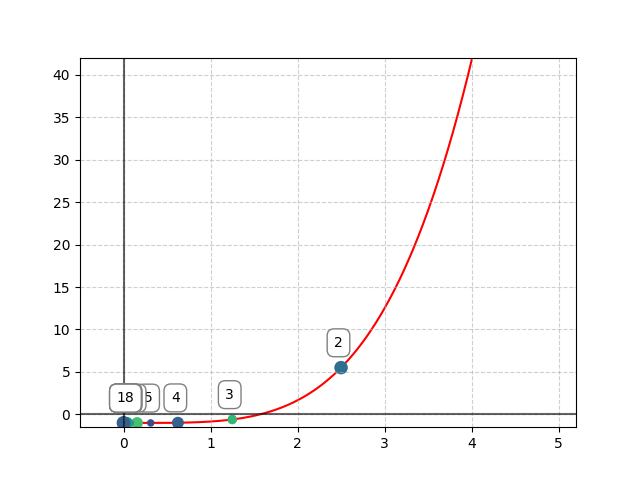
\includegraphics[scale=0.8]{img/bisection.png}
  \caption{Intervalo dalijimo pusiau algoritmo veikimo rezultatai.}
  \label{img:bisection}
\end{figure}

\begin{figure}[H]
  \centering
  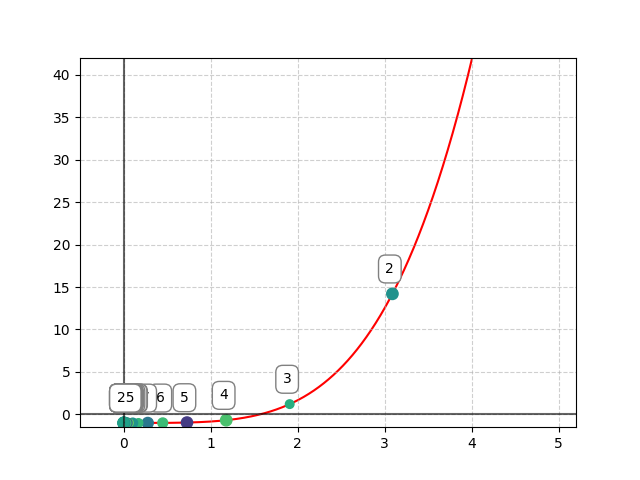
\includegraphics[scale=0.8]{img/golden-section.png}
  \caption{Auksinio pjūvio algoritmo veikimo rezultatai.}
  \label{img:golden-section}
\end{figure}

\begin{figure}[H]
  \centering
  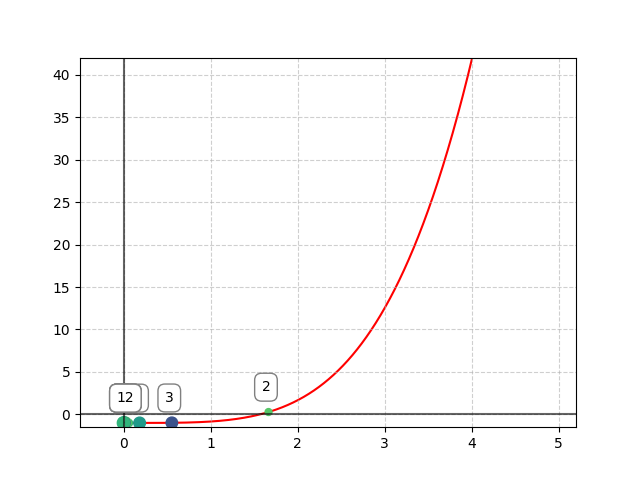
\includegraphics[scale=0.8]{img/newtons.png}
  \caption{Niutono metodo algoritmo veikimo rezultatai.}
  \label{img:newtons}
\end{figure}

\end{document}
